\section{Pipeline}\label{appendix:pipeline}
As shown in \cref{fig:pipeline}, our pipeline consists of two main training stages. (1) The SFT training stage first generates initial solutions that are validated through execution feedback, followed by critique generation where the generator learns to provide critiques based on execution feedback. These components are then used to train the final critic model through supervised finetuning. (2) The RL training stage leverages the critic's feedback to guide the generator in producing improved solutions, which are validated in a sandbox environment.

\begin{figure*}[h!]
    \centering
    \includegraphics[width=\linewidth]{figs/pipeline_v2.pdf}
    \vspace{-40mm}
    \caption{Overview of our two-stage training pipeline {\ours}.}
    \label{fig:pipeline}
\end{figure*}


\section{Supplementary Discussion of Related Work}\label{appendix:related}
\cref{tab:related_comparison} categorizes prior methods into reward models, generative reward models, and critic models. Reward models like Standard RM~\cite{bradley1952rank} and SynRM~\cite{ye2024improving} focus on discrimination by outputting scalar rewards $r$ but lack refinement or critique supervision. Generative reward models, such as CLoud~\cite{ankner2024critique} and Critic-RM~\cite{yu2024self}, enhance discrimination by producing both rewards $r$ and critiques $c$, but their critiques primarily serve as a by-product for rewards rather than actionable refinement suggestions. Critic models, including UltraCM~\cite{cui2023ultrafeedback}, Shepherd~\cite{wang2023shepherd}, and CriticGPT~\cite{mcaleese2024llm}, focus on generating critiques but rely heavily on human-annotated critique data, which limits scalability. In contrast, {\ours} unifies discrimination and refinement by generating actionable critiques without direct supervision, leveraging execution feedback and reinforcement learning to enable scalable, iterative improvement.




\newcolumntype{g}{>{\columncolor{green!10}}c}
\setlength\tabcolsep{7pt}
\begin{table}[htbp]
\centering
\huge
\newcolumntype{b}{>{\columncolor{blue!10}}c}
\renewcommand{\arraystretch}{1.6}
\resizebox{0.5\textwidth}{!}{

\begin{tabular}{lccccc}

\toprule
\multicolumn{1}{c}{\multirow{2}{*}{Method}} & \multicolumn{4}{c}{Data Quality} &  \\ \cline{2-6} 
\multicolumn{1}{c}{}                       & Nums.       & Cons.    & Avg Attr.      & Synt.    \\ \midrule
IFeval~\cite{zhou2023instruction} & 541  & H & 1.54 & \ding{51} \\
FollowBench~\cite{jiang2023followbench} & 820 & H/S & 3.0 & \ding{51}  \\
CFBench~\cite{zhang2024cfbench} & 1000 & H/S & 4.24 & \ding{55} \\
InFoBench~\cite{qin2024infobench} & 500 & H/S & 4.5 & \ding{55} \\
\our (FineWeb Split) & 6159 & H/S & \textbf{45.9} & \ding{55} \\
\our (Multi-source Split) & 1600 & H/S & \textbf{29.9} & \ding{55} \\
\bottomrule
\end{tabular}%
}
\caption{
  Detailed comparison of relevant works. Ours
represents our dataset construction approach. \textquotesingle Nums.\textquotesingle, \textquotesingle Cons.\textquotesingle, \textquotesingle Avg Attr.\textquotesingle,
and \textquotesingle Synt.\textquotesingle\  denote the number of samples, constraint types, average number of attributes, and whether the data is synthesized.
}


  \label{tab:comparison}
\end{table}










\section{Implementation Details}
\subsection{Simulation}\label{appendix:simulation}
In our simulation (\cref{sec:preliminary}), we model the iterative refinement process using a Markov chain with parameters $p_{\mathrm{init}}$, $p_{\mathrm{cc}}$, and $p_{\mathrm{cw}}$ to represent the initial correctness, the probability of maintaining correctness, and the probability of turning incorrect solutions correct, respectively. Critiquing ability is controlled by varying $p_{\mathrm{cc}}$ and $p_{\mathrm{cw}}$ (e.g., strong critiquing: $p_{\mathrm{cc}}=0.9$, $p_{\mathrm{cw}}=0.3$; weak critiquing: $p_{\mathrm{cc}}=0.7$, $p_{\mathrm{cw}}=0.15$), while discrimination ability is adjusted via true positive rate (TPR) and false positive rate (FPR) (e.g., strong discrimination: $\mathrm{TPR}=0.7$, $\mathrm{FPR}=0.2$; weak discrimination: $\mathrm{TPR}=0.6$, $\mathrm{FPR}=0.3$). For each setting, we simulate $n$ refinement steps using Python, generating solutions based on refinement probabilities, applying a classifier to predict correctness, and selecting the best solution from predicted correct ones. The results are computed over 50,000 iterations and plotted to analyze the impact of critiquing and discrimination on final success rates.
Specifically, the two processes\,---\,only using discrimination and using both discrimination and critiquing\,---\,are illustrated in \cref{fig:graphical} to provide a clearer understanding of our simulation setup.

\begin{figure}[h!]
    \centering
    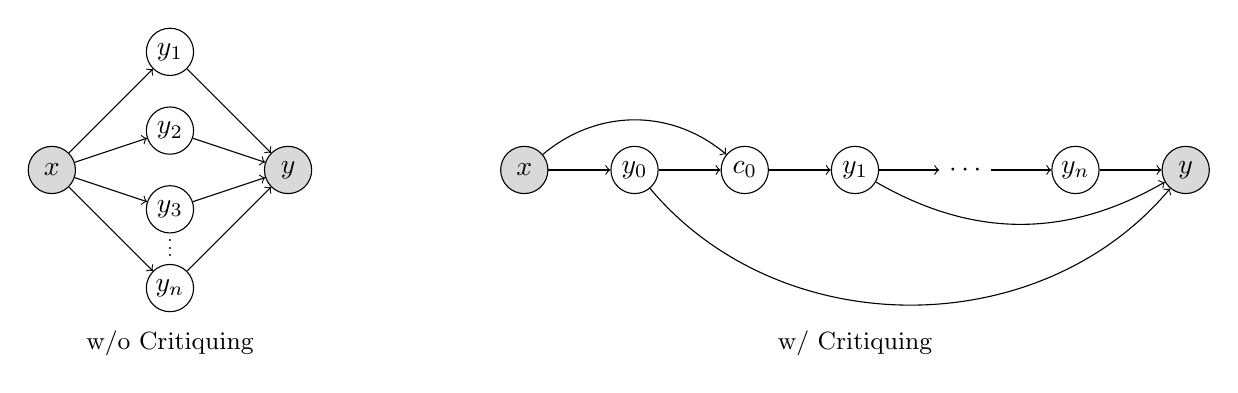
\begin{tikzpicture}[
        node distance=1.2cm,
        state/.style={circle,draw,minimum size=0.6cm,inner sep=0pt},
        gray/.style={fill=gray!30}
    ]
        \node[state,gray] (c1) at (0,0) {$x$};
        \node[state] (x11) at (1.5,1.5) {$y_1$};
        \node[state] (x12) at (1.5,0.5) {$y_2$};
        \node[state] (x13) at (1.5,-0.5) {$y_3$};
        \node[state] (x1n) at (1.5,-1.5) {$y_n$};
        \node[state,gray] (x1) at (3,0) {$y$};
        
        \draw[->] (c1) -- (x11);
        \draw[->] (c1) -- (x12);
        \draw[->] (c1) -- (x13);
        \draw[->] (c1) -- (x1n);
        \draw[->] (x11) -- (x1);
        \draw[->] (x12) -- (x1);
        \draw[->] (x13) -- (x1);
        \draw[->] (x1n) -- (x1);
        
        \node[scale=0.7] at (1.5,-0.92) {$\vdots$};
        
        \node[state,gray] (c2) at (6,0) {$x$};
        \node[state] (x20) at (7.4,0) {$y_0$};
        \node[state] (f1) at (8.8,0) {$c_0$};
        \node[state] (x21) at (10.2,0) {$y_1$};
        \node (dots) at (11.6,0) {$\cdots$};
        \node[state] (x2n) at (13,0) {$y_n$};
        \node[state,gray] (x2) at (14.4,0) {$y$};
        
        \draw[->] (c2) -- (x20);
        \draw[->] (x20) -- (f1);
        \draw[->] (f1) -- (x21);
        \draw[->] (x21) -- (dots);
        \draw[->] (dots) -- (x2n);
        \draw[->] (x2n) -- (x2);
        \draw[->] (c2) to[bend left=40] (f1);
        
        \draw[->] (x20) to[bend right=50] (x2);
        \draw[->] (x21) to[bend right=30] (x2);
        
        \node at (1.5,-2.2) {\small w/o Critiquing};
        \node at (10.2,-2.2) {\small w/ Critiquing};
    \end{tikzpicture}
    \caption{Graphical models for refinement processes: (left) only using discrimination (best-of-$n$ sampling) and (right) using both discrimination and critiquing (sequential critique-revision).}
    \label{fig:graphical}
\end{figure}

\subsection{Prompt Templates}\label{appendix:prompt}
\paragraph{Critique-revision.} The generator model $\pi(y \mid x)$ is implemented as a simple zero-shot generation process, where the model generates a solution $y$ directly from the problem statement $x$ without additional context or feedback. The critic model $Q_\theta(c \mid x, y)$, as described in the main paper, generates textual feedback $c$ using a structured prompt that incorporates the problem $x$, the solution $y$, and explicit instructions to provide actionable and formatted suggestions. The improved solution distribution $\pi(y \mid x, y^\prime, c)$ is implemented as a two-turn process: in the first turn, the generator model drafts the initial solution $y^\prime$ conditioned on the problem $x$ as the user message; in the second turn, the critique $c$ is presented as the user message, and the model revises the solution, conditioned on $x$, $y^\prime$, and $c$.

\paragraph{Execution-guided Critique Generation.}
To generate high-quality critiques~(\cref{sec:sft}), we leverage execution feedback from a sandbox environment that evaluates the initial solution $y^\prime$ against the test cases $T$ for the problem $x$. The execution results are mapped to predefined hint templates, which guide the critique generation process. The critic model is prompted with a structured template incorporating the problem $x$, the solution $y^\prime$, and the corresponding hint $h$, enabling it to produce actionable and context-aware feedback. To prevent hallucination, critiques that explicitly reference the hints are filtered out. This ensures that the generated critiques are grounded in observable failures while effectively supporting solution refinement.

\begin{table}[h!]
\begin{tcolorbox}[
    colback=gray!5,
    colframe=gray!75,
    title=Prompt Template for Critique Generation,
    fonttitle=\bfseries
]
\begin{lstlisting}[
    basicstyle=\scriptsize\ttfamily,
    breaklines=true,
    postbreak=\mbox{\textcolor{gray}{$\hookrightarrow$}\space}
]
You are tasked with analyzing an answer to a problem and providing constructive feedback. Do NOT provide direct solutions.

Problem description:
<problem>
{problem}
</problem>

Answer:
<answer>
{answer}
</answer>

Structure your response using the following format (without <format> tags):
<format>
Analysis:
{{Analysis}}

Improvement suggestions:
{{Suggestions}}

Overall judgment: {{Correct/Incorrect}}
</format>
\end{lstlisting}
\end{tcolorbox}
\end{table}

\begin{table}[h!]
\begin{tcolorbox}[
    colback=gray!5,
    colframe=gray!75,
    title=Prompt Template for Execution-guided Critique Generation,
    fonttitle=\bfseries
]
\begin{lstlisting}[
    basicstyle=\scriptsize\ttfamily,
    breaklines=true,
    postbreak=\mbox{\textcolor{gray}{$\hookrightarrow$}\space}
]
You are tasked with analyzing an answer to a problem and providing constructive feedback. Do NOT provide direct solutions.
Please carefully reason about the hint to guide the user.
**Important: Do NOT mention 'the hint' in your feedback.**

Problem description:
<problem>
{problem}
</problem>

Answer:
<answer>
{solution}
</answer>

Hint:
<hint>
{hint}
</hint>

Structure your response using the following format (without <format> tags):
<format>
Analysis:
{{Analysis}}

Improvement suggestions:
{{Suggestions}}

Overall judgment: {{Correct/Incorrect}}
</format>
\end{lstlisting}
\end{tcolorbox}
\end{table}


\begin{table}[t!]
\centering
\small
\rowcolors{2}{gray!10}{white} %
\caption{Mapping between execution results and hint templates used for critique synthesis.}
\label{tab:hint}
\vspace{3mm}
\begin{tabular}{p{2.3cm}p{5cm}}
\toprule
Execution Result      & Hint                                                                                                                                  \\
\midrule
Success (100\%)             & The draft solution is correct. A concise and positive feedback is recommended.                                                        \\
Failure (0\%) & The draft solution is entirely wrong. A concise feedback requesting a fresh restart is recommended.               \\
Partial Success            & \parbox{5cm}{Input:\\
                         \{input\}\\
                         \\
                         Expected Output:\\
                         \{expected\_output\}\\
                         \\
                         Actual Output:\\
                         \{actual\_output\}} \\
Runtime Error  & \parbox{5cm}{The code block:\\
                         ```python\\
                         \{code\_block\}\\
                         '''\\
                         raised \{error\}.}                             \\
\bottomrule
\end{tabular}
\end{table}

\subsection{Training}\label{appendix:training_details}
\paragraph{Data Curation.} Our data curation process starts with the TACO dataset~\cite{li2023taco} and handles both function-based and input-output-based programming problems. We filter out malformed problems by removing those containing image tags and unusual HTML spans. For unit tests, we process them differently based on their type: function-based tests are converted to assertion statements, while input-output tests are standardized into a sandbox format with stdin-stdout pairs. We exclude problematic unit tests such as those with malformed string inputs (containing assignments or unexpected list operations) or invalid function calls.
To avoid contamination, we further exclude 47 problems that overlap with our evaluation benchmarks.
The final dataset is deduplicated based on problem descriptions, resulting in 18,820 problems.

\paragraph{Supervised Finetuning.} 
We leverage the synthesized critiques to perform supervised finetuning (SFT) on the model, enabling it to generate improved solutions. For each problem, we sample one initial solution and one corresponding synthesized critique, and train the model on these problem-solution-critique pairs. The training process follows the hyperparameters outlined in \cref{tab:sft_hyper}.

\paragraph{RL Training.}
We use VeRL~\cite{sheng2024hybridflow} as the codebase to optimize the model's generation quality. During RL training, we sample 4 initial solutions for each problem and train the critic model on all corresponding problem-solution pairs. This approach helps mitigate overfitting by exposing the critic to a diverse set of solutions for each problem. The RL training process follows the hyperparameters outlined in \cref{tab:rl_hyper}.


\begin{minipage}{0.48\textwidth}
    \begin{table}[H]
    \small
    \centering
    \caption{SFT Hyperparameters.}
    \label{tab:sft_hyper}
    \vspace{3mm}
    \begin{tabular}{ll}
    \toprule
    \textbf{Parameter}           & \textbf{Value}      \\ \midrule
    Learning Rate                & 2 $\times$ 10\textsuperscript{-5} \\
    Learning Rate Schedule       & Cosine             \\
    Training Batch Size         & 256                \\
    Maximum Token Length         & 2,048              \\
    Training Epochs              & 1                  \\
    Mixed Precision Format       & bfloat16           \\ \bottomrule
    \end{tabular}
    \end{table}
\end{minipage}
\hfill
\begin{minipage}{0.48\textwidth}
    \begin{table}[H]
    \small
    \centering
    \caption{RL Hyperparameters.}
    \label{tab:rl_hyper}
    \vspace{3mm}
    \begin{tabular}{ll}
    \toprule
    \textbf{Parameter}           & \textbf{Value}      \\ \midrule
    Training Batch Size          & 1,024              \\
    Mini-Batch Size          & 256                \\
    Group Size & 8 \\
    Learning Rate                & 1 $\times$ 10\textsuperscript{-5} \\
    KL Coefficient               & 0.001              \\
    Maximum Prompt Length        & 1,536              \\
    Maximum Response Length      & 768                \\
    Temperature & 1.0 \\
    Training Epochs              & 2                  \\ \bottomrule
    \end{tabular}
    \end{table}
\end{minipage}

\subsection{Evaluation.}\label{appendix:evaluation_details}

\paragraph{Inference.} 
During inference, we use a temperature of 0.7 for generating both initial solutions and critiques, while revised solutions are generated using greedy decoding. The maximum number of tokens generated is set to 1,024 for all stages. 

\paragraph{Reward Calculation.} 
To calculate rewards for our JudgeBench evaluation (\cref{sec:judgebench_exp}), we use a critic model to assess the quality of solutions. Specifically, we generate multiple critiques for each solution and aggregate the results through majority voting. For each solution pair, the critic model compares the frequency of being labeled as ``Correct'' to determine which solution is better. As shown in \cref{fig:judgebench_scaling}, we find that the accuracy of this majority voting strategy improves as the number of votes increases.

\paragraph{Code Similarity Calculation.}
To measure code similarity while accounting for semantically equivalent code with different variable names, we follow \citep{zheng2024makes} and implement a two-step comparison approach. We first normalize the code by parsing it into an Abstract Syntax Tree (AST), systematically renaming variables to canonical forms, and converting back to consistently formatted text. We then compute a similarity ratio using Python's \texttt{difflib.SequenceMatcher}, which represents the proportion of matching characters in the optimal alignment of the two normalized code sequences. This approach yields a score between 0 and 1, allowing us to identify structurally similar solutions regardless of variable naming choices.



\begin{figure}[ht]
    \centering
    \subfigure[The effect of the number of votes on the accuracy of majority voting in reward calculation. As the number of votes increases, the accuracy improves significantly, demonstrating the scalability and robustness of the majority voting approach.]{
        \includegraphics[width=0.45\textwidth]{figs/judgebench_scaling.pdf}
        \label{fig:judgebench_scaling}
    }
    \hfill
    \subfigure[Training curve of the value network in PPO, showing the mean predicted value over training steps.]{
        \includegraphics[width=0.45\textwidth]{figs/value_curve.PNG}
        \label{fig:value_curve}
    }
    \caption{(a) Majority voting accuracy improvement with increasing votes. (b) Training curve of the value network.}
    \label{fig:combined_figures}
\end{figure}

\section{The Credit Assignment Issue for Critic Training}\label{appendix:credit_assignment}
Our initial attempts to train critics using Proximal Policy Optimization~\cite{schulman2017proximal} for RL training revealed challenges in credit assignment for critique generation, as evidenced by the unstable value predictions shown in \cref{fig:value_curve}. This difficulty arises because the quality of a critique is inherently holistic\,---\,it depends on multiple interdependent aspects like accuracy, completeness, and constructiveness\,---\,making it hard for the value network to learn which parts of the generated critique contributed to the final reward. These observations motivated our switch to GRPO, which circumvents the value prediction problem by using Monte Carlo sampling to directly estimate advantages, leading to more reliable credit assignment without the need for a potentially unstable value network.

\section{{\ours} Samples}\label{appendix:samples}
In \cref{tab:cc_sample,tab:lcb_sample,tab:mbppplus_sample}, we present sample critiques generated by {\ours} for solutions provided by Qwen2.5-Coder.



\renewcommand{\arraystretch}{1.4} %

\lstset{
    basicstyle=\ttfamily\scriptsize,
    breaklines=true,
    frame=single,
    backgroundcolor=\color{lightgray!20},
    showstringspaces=false
}

\newpage

\begin{table}[]
    \centering
    \small
    \caption{A sample problem from CodeContests~\cite{li2022competition}, with by the solution generated by Qwen2.5-Coder and the critique provided by the {\ours} critic.}
    \label{tab:cc_sample}
\begin{longtable}{m{0.45\textwidth}m{0.45\textwidth}}
\toprule
\textbf{Problem \& Solution}  &
\textbf{Critique} \\ 
\midrule
\begin{lstlisting}[frame=none,
    backgroundcolor=\color{white},
    numbers=none,
    xleftmargin=0pt,
    framexleftmargin=0pt,
    framexrightmargin=0pt,
    framextopmargin=0pt,
    framexbottommargin=0pt]
You had n positive integers a_1, a_2, ..., a_n arranged in a circle. For each pair of neighboring numbers (a_1 and a_2, a_2 and a_3, ..., a_{n - 1} and a_n, and a_n and a_1), you wrote down: are the numbers in the pair equal or not.

Unfortunately, you've lost a piece of paper with the array a. Moreover, you are afraid that even information about equality of neighboring elements may be inconsistent. So, you are wondering: is there any array a which is consistent with information you have about equality or non-equality of corresponding pairs?
\end{lstlisting}


\begin{lstlisting}[language=python]
def can_form_array(s):
    n = len(s)
    # We will try to assign values to the array a
    # Start with assigning 1 to the first element
    a = [1] * n
    
    # Try to assign values based on the given conditions
    for i in range(n):
        if s[i] == 'E':
            a[(i + 1) %
        else:
            a[(i + 1) %
    
    # Check if the last and first elements are consistent with s[n-1]
    if s[-1] == 'E' and a[0] != a[-1]:
        return "NO"
    if s[-1] == 'N' and a[0] == a[-1]:
        return "NO"
    
    return "YES"

def main():
    import sys
    input = sys.stdin.read().splitlines()
    t = int(input[0])
    results = []
    for i in range(1, t + 1):
        s = input[i]
        results.append(can_form_array(s))
    
    for result in results:
        print(result)

if __name__ == "__main__":
    main()
\end{lstlisting} 
&
\begin{lstlisting}[frame=none,
    backgroundcolor=\color{white},
    numbers=none,
    xleftmargin=0pt,
    framexleftmargin=0pt,
    framexrightmargin=0pt,
    framextopmargin=0pt,
    framexbottommargin=0pt]
Analysis:
The provided solution attempts to construct an array based on the sequence of 'E' and 'N' but does not correctly handle the circular nature of the array and the constraints imposed by these characters. Specifically, the approach does not ensure consistency across the entire circular arrangement, particularly at the boundary where the last element connects back to the first.

The code assigns values to the array elements based on whether the current character is 'E' or 'N', but it does not account for potential conflicts that arise when the array wraps around. This means that the final check between the first and last elements might fail due to inconsistencies introduced earlier in the array construction process.

Improvement suggestions:
1. Consider using a more systematic approach to handle the circular nature of the array. One possible method is to use a graph traversal algorithm, treating each position in the array as a node and each 'E' or 'N' as an edge with a label indicating equality or inequality.
2. Use a union-find data structure to manage equivalence classes of indices that must hold the same value due to 'E' connections.
3. Iterate through the string and apply the rules: if 'E', ensure the indices are in the same set; if 'N', ensure they are in different sets.
4. After processing the string, verify that no conflicts exist in the union-find structure, particularly focusing on the circular connection between the first and last elements.
5. If no conflicts are found, it is possible to construct an array that satisfies the conditions; otherwise, it is not.

Overall judgment: Incorrect
\end{lstlisting}
\\ 
\bottomrule
\end{longtable}
\end{table}


\newpage

\begin{table}[]
    \centering
    \small
    \caption{A sample problem from LiveCodeBench~\cite{jain2024livecodebench}, with by the solution generated by Qwen2.5-Coder and the critique provided by the {\ours} critic.}
    \label{tab:lcb_sample}
\begin{longtable}{m{0.45\textwidth}m{0.45\textwidth}}
\toprule
\textbf{Problem \& Solution}  &
\textbf{Critique} \\ 
\midrule
\begin{lstlisting}[frame=none,
    backgroundcolor=\color{white},
    numbers=none,
    xleftmargin=0pt,
    framexleftmargin=0pt,
    framexrightmargin=0pt,
    framextopmargin=0pt,
    framexbottommargin=0pt]
You are given a binary string s and an integer k.
A binary string satisfies the k-constraint if either of the following conditions holds:

The number of 0's in the string is at most k.
The number of 1's in the string is at most k.

Return an integer denoting the number of substrings of s that satisfy the k-constraint.
\end{lstlisting}

\begin{lstlisting}[language=python]
class Solution:
    def countKConstraintSubstrings(self, s: str, k: int) -> int:
        def count_substrings_with_max_char(s, max_char, k):
            left = 0
            count = 0
            current_count = 0
            result = 0
            
            for right in range(len(s)):
                if s[right] == max_char:
                    current_count += 1
                
                while current_count > k:
                    if s[left] == max_char:
                        current_count -= 1
                    left += 1
                
                result += right - left + 1
            
            return result
        
        count_0s = count_substrings_with_max_char(s, '0', k)
        count_1s = count_substrings_with_max_char(s, '1', k)
        
        return count_0s + count_1s
\end{lstlisting}
 &
\begin{lstlisting}[frame=none,
    backgroundcolor=\color{white},
    numbers=none,
    xleftmargin=0pt,
    framexleftmargin=0pt,
    framexrightmargin=0pt,
    framextopmargin=0pt,
    framexbottommargin=0pt]
Analysis:
The provided solution attempts to solve the problem by counting substrings based on the maximum occurrence of '0' and '1' up to `k`, but it does not correctly account for all possible substrings that satisfy the k-constraint. The approach incorrectly calculates the intersection of substrings that satisfy both conditions without properly considering the overlap between these substrings. Additionally, the logic for counting substrings is flawed as it does not consider every possible substring of `s`; instead, it focuses on contiguous sequences of '0's and '1's up to `k`.

Improvement suggestions:
1. **Re-evaluate the Approach**: Instead of focusing on contiguous sequences of '0's and '1's, the solution should consider every possible substring of `s` and check if it satisfies the k-constraint.
2. **Iterate Over All Substrings**: Use nested loops to iterate over all possible substrings of `s`. For each substring, count the occurrences of '0' and '1' and check if either count is less than or equal to `k`.
3. **Count Valid Substrings**: Maintain a counter to keep track of how many substrings meet the k-constraint criteria.
4. **Simplify the Logic**: Consider using Python's slicing capabilities to easily extract and evaluate each substring without unnecessary checks for contiguous characters.

Overall judgment: Incorrect
\end{lstlisting}
\\ 
\bottomrule
\end{longtable}
\end{table}


\newpage

\begin{table}[]
    \centering
    \small
    \caption{A sample problem from MBPP+~\cite{liu2024your}, with by the solution generated by Qwen2.5-Coder and the critique provided by the {\ours} critic.}
    \label{tab:mbppplus_sample}
\begin{longtable}{m{0.45\textwidth}m{0.45\textwidth}}
\toprule
\textbf{Problem \& Solution}  &
\textbf{Critique} \\ 
\midrule
\begin{lstlisting}[frame=none,
    backgroundcolor=\color{white},
    numbers=none,
    xleftmargin=0pt,
    framexleftmargin=0pt,
    framexrightmargin=0pt,
    framextopmargin=0pt,
    framexbottommargin=0pt]
Write a python function to check whether every odd index contains odd numbers of a given list.
\end{lstlisting}


\begin{lstlisting}[language=python]
def odd_length_sum(arr):
    n = len(arr)
    res = 0
    
    # Iterate through each element in the array
    for i in range(n):
        # Calculate the number of subarrays in which arr[i] is present
        count = ((i + 1) * (n - i) + 1) // 2
        
        # If the count is odd, add the element to the result
        if count %
            res += arr[i]
    
    return res
\end{lstlisting} 
&
\begin{lstlisting}[frame=none,
    backgroundcolor=\color{white},
    numbers=none,
    xleftmargin=0pt,
    framexleftmargin=0pt,
    framexrightmargin=0pt,
    framextopmargin=0pt,
    framexbottommargin=0pt]
Analysis:
The provided solution checks if the parity (odd/even nature) of the numbers at odd indices matches the index itself. This means it verifies that a number at an odd index is odd, and a number at an even index is even. However, this does not correctly address the problem at hand, which requires checking whether every odd index contains an odd number, not just matching the parity of the index.

Improvement suggestions:
- Review the logic used in the function. Instead of checking if the parity of the number matches the parity of the index, the function should directly check if the number at each odd index is odd.
- Consider using a more straightforward loop or list comprehension to achieve the desired result.

Overall judgment: Incorrect
\end{lstlisting}
\\ 
\bottomrule
\end{longtable}
\end{table}



























    
    
    
    
    
    
    
    
    
    
    
    
    

    
    
    
    
    
    
    
    
    
    
    
    


    
    
    
    
    

























































































